\documentclass{article}
\usepackage{multicol}
\usepackage{titlesec}
\usepackage[margin=0.75in]{geometry}
\usepackage{pgfplots}
\usepackage{array}
% MACROS %

\titleformat{\section}
  {\large\scshape\filcenter}{\thesection}{}{}
\graphicspath{ {pretty_code/} }

\begin{document}

\title{\textbf{Optimal Scheduling of Introductory Programming Lab}}
\author{
   Chris Alfino \textit{\&} Rajan Selvan\\
   \vspace{12pt}
   \small\textit{Math 480}\\
   Connor Moore\\
   \small\textit{CSE TA Coordinator}}
\date{}

\maketitle
\renewcommand{\abstractname}{}
\begin{abstract}
Teaching assistant coordinators for the introductory computer science courses at the UW wish to determine staffing assignments for the introductory programming lab, a tutoring lab for students in CSE 142 and 143. Our goal was to assign every teaching assistant to a certain number of lab time slots across the week. Two sets of considerations are accounted for: TA work schedule preferences and staffing requirements determined by the CSE department. We apply standard linear programming techniques to this assignment problem, generating solutions in a manner that will scale with the constantly growing TA numbers in UW CSE. Finally, we provide a simulation tool to automate evaluation of future schedules and various other lab management policies.
\end{abstract}

\noindent\makebox[\linewidth]{\rule{\textwidth}{0.4pt}}

\setlength\columnsep{0.45in}
\setlength{\parskip}{0.5em}
\begin{multicols}{2}

\section*{Background}

In recent years, enrollment in the University of Washington's introductory computer science classes, CSE 142 and CSE 143, has skyrocketed. Students are interested in programming for a variety of reasons; industry and academic research positions abound, while programming skills are becoming increasingly necessary in other disciplines around campus. In Winter 2014, CSE 142 and 143 each hit new enrollment records: 810 and 530 students respectively! In order to meet new demand, CSE 142 and 143 have needed to scale their educational efforts. Requisite hiring of undergraduate teaching assistants has increased in proportion with enrollment, with each TA-lead discussion section containing roughly 20 students.

The introductory programming lab (IPL) in Mary Gates Hall is a two room computer lab open from 12:30pm to 9:30pm every week day and from 1:30pm to 3:30pm on Saturday and Sunday. Students in CSE 142 and 143 can come to the lab during these hours to be helped with conceptual and homework questions by whichever TAs are currently staffed. A queuing system in the lab allows students to add themselves to a help queue through a web interface. The process for a working TA is then straightforward: he or she dequeues a student and helps the student one-on-one for 2 to 10 minutes. A TA typically signs up for 2 one-hour schedule slots each week, so that the number of TAs in the lab ranges from as few as 1 or 2 on weekends to as many as 7 on busy weekday evenings.

As it stands, the CSE department's approach to IPL staffing is not scalable. At a meeting with all sixty-seven TAs in attendance, the TA coordinators display the entire IPL schedule up on a projector screen and proceed to call on each TA in order from most to least senior. Each TA responds with his or her top choice among time slots not taken, and the TA coordinator tentatively schedules that choice. Toward the end of the process, when younger TAs are predictably choosing from among the least popular time slots, conflicts inevitably arise. Resolution usually requires that TAs volunteer to swap assignments, and coordinators negotiate the schedule switches in real time. The approach is ultimately effective, but fails to capture more nuanced TA preferences and becomes increasingly unmanageable with large TA numbers.

\section*{Objective}

At a high level, \textit{our goal was to schedule TA IPL shifts such that minimum and maximum staffing requirements are met and TA preferences are accommodated as much as possible}. The CSE department has a number of easily formalized requirements for staffing, including minimum numbers of total and senior TAs required for each time slot. A \textit{senior TA} is a TA who has instructed for at least three quarters. For our main problem, we assumed that the department's quotas for TAs at each time slot were set in stone.

TAs have some preferences that cannot be ignored in scheduling hours. Each student has hours that they cannot work (during class, for instance), and also preferences about when they'd like to work. As a goal, we would like to maximize TA preference accommodation, splitting ties according to TA seniority (number of quarters taught). These preferences must be balanced, however, with the need to compose groups of ideally mixed seniority during key hours. Before a particularly tough CSE 143 assignment, it is essential that more experienced TAs are present to field questions and help less experienced TAs. These factors are weighed into our mathematical objective in a way that is customizable in the future.

As a stretch goal, we sought to provide a simulation tool to model IPL queue behavior with the hope that such a tool would provide a way to evaluate different sets of staffing requirements. A good set of quotas minimizes queue response time, but the problem is complicated by various factors: how much does the presence of senior TAs affect service time? what is the best dequeuing policy when faced with 2-minute and 10-minute queues that are both full? The CS department has already done some work to accommodate varying student demand across the week. More students arrive at the IPL during the hours before important due dates, for instance, so more TAs are staffed during these hours. Fortunately over the past couple years, data about the frequency of CSE 142 and 143 student questions at various times of the day has been collected.

\section*{Basic LP}
Our main problem can be formulated as a general assignment problem, with $m$ TAs and $n$ time slots. Under this formulation, we let $x_{ij}$ be a 0-1 variable where $x_{ij} = 1$ if TA $i$ works time slot $j$ and $x_{ij} = 0$ otherwise.

For each TA $i$, let $s_i = 1$ if TA $i$ is a senior TA, 0 otherwise. Each TA must work at least two hours each week and can work up to a self-imposed maximum $m_i$ hours. As undergraduate UW employees, TAs cannot legally work more than 19.5 hours. Formally for each TA $i$,

\begin{equation}
2 \leq \sum_{j=1}^{n}x_{ij} \leq \textrm{min}(m_i, 19.5).
\end{equation}

Time slot preferences introduce additional constraints. Real numbers $a_{ij} \in [0,1]$ represent the availability preference of TA $i$ at slot $j$, with larger $a_{ij}$ indicating greater preference. In addition, we encode absolute unavailability as a preference value below some threshold $a_{min}$. If $a_{ij} \leq a_{min}$, TA $i$ \textit{cannot} work time slot $j$, and so should not be scheduled for that slot. For each such $a_{ij}$, we impose the constraint
\begin{equation}
x_{ij} = 0.
\end{equation}

Now for each time slot $j$, let $t_j$ and $u_j$ be the minimum number of total and senior TAs respectively required. Let $T_j$ be the maximum number of TAs allowed for each time slot. Formally for each time slot $j$,

\begin{equation}
t_j \leq \sum_{i=1}^{m}x_{ij} \leq T_j
\end{equation}

\begin{equation}
u_j \leq \sum_{i=1}^{m}x_{ij}s_i.
\end{equation}

Unlike a general assignment problem, we are not simply minimizing TA usage. After all, TAs may in fact \textit{wish} to work more hours, and since the CSE department has money to spare on staffing costs, we can assume that the department is willing to pay to staff as many as $T_j$ TAs in each slot. The total adherence to the preferences of TA $i$ is:

\begin{equation}
a(i) = \sum_{j=1}^na_{ij}x_{ij}.
\end{equation}
For each TA $i$, let $q_i$ be the number of quarters that TA has taught (a measure of seniority). We give priority to seniors using a customizable weight $w \in [0,1]$, linearly mapping $w$ values to priority coefficients between $[1, q_i + 1]$. Our objective function is a measure of total TA preference, weighted by TA seniority:

\begin{equation}
\textrm{maximize } z = \sum_{i=1}^m(wq_i + 1)\cdot a(i).
\end{equation}

\section*{LP Implementation}

Sage's \texttt{MixedIntegerLinearProgram} precisely fits our needs. Each constraint above translates immediately to a block of code in the short Sage script \texttt{lp.sage}. The formulation coded there uses the values mentioned above, but makes use of three important data input sets: staff quotas, preference lists, and seniority measurements. We focused our research on the Autumn 2014 term, so all of our data sets (both generated and gathered) are based on that quarter.

Staff quotas vary considerably quarter-to-quarter and are typically determined by assuming that each TA will work two hours a week. The department loosely distributes $2n$ working hours across the week according to student question frequency. Table 1 shows the quotas from Autumn 2014 that we used for our LP solution. Of note is the spike on Thursday afternoons, a consequence of the CSE 143 assignment due time. Unsurprisingly, the most difficult requests often come from 143 students right before their due dates, so the department concentrates senior TA quotas around this period as well.

Random, plausible TA preference generation was a more involved process. As described above, complete TA preferences are only approximated in the current assignment system and have never been collected from TAs with the numerical precision of the $a_{ij}$ values in our LP. In future terms, the department will need to collect this information using some kind of survey. For testing purposes, we attempted to generate random preference lists for each TA, capturing the following trends:
\begin{itemize}
   \item TAs likely have a top time slot that they'd like to work on any given day. Generally, working a time slot closer to this slot is preferable.
   \item TAs likely have a ranking of preferable days in mind (e.g. Wednesday, Monday, etc. from most to least preferable).
   \item Since most TAs are taking three or four classes per term, each will have hours that they absolutely cannot work.
\end{itemize}

The Python code for preference generation is found in the functions of \texttt{preferences.py}.

For each TA, we generate a preference map like the one shown in Figure 1. Python's built-in \texttt{gammavariate} function gives us a satisfactory distribution across each day, visible in the gradual variation across days. We zero-out several hours across the week to imitate a typical UW undergraduate course schedule. And finally, we multiply each day's preferences by a random rank coefficient, since it is unlikely that a TA would prefer all days equally. As a final step, the map is transformed into a complete preference list where the $j$th entry corresponds to the $j$th time slot in the LP: a vector $[a_{i1}, ... a_{i(m-1)}]$ for TA $i$.

As mentioned above, TA seniority is measured in number of quarters taught. These values were provided by the CSE department and read into our Sage program as a simple list of integers. Because TA preferences are randomly generated, the pairing of seniority value to preference list was done arbitrarily.

\section*{LP Simplifications}

Our LP formulation captures many of the constraints that the CSE department imposes on scheduling, but makes several key simplifications.

Except for the minimum TA quotas per time slot ($t_j$ values above), the LP does not encode department preferences for which time slots it would prefer TAs to work extra hours. Minimum values, as it stands, are calculated assuming each TA will work 2 hours a week. But supposing a TA would like to work 3 or 4 hours instead, these extra hours are placed entirely according to the TAs preference. The essential simplification is that coordinators do not actually specify \textit{real-valued relative preferences} for how many TAs they'd like to work any given time slot, but instead can only specify bounds.

Random preference generation, despite the efforts described above, is still overly simplified. We assume in the generation code that each TA essentially has a ``favorite'' time per week and would prefer hours closer to this slot. But favorite time slots are surely not uniformly random across the TA community; most TAs would likely avoid the IPL shifts around dinner time or in the late evening, for instance. A better representation of typical TA preference would account for subtler distributions of preference across the day and week.

And our scheme for preference reporting is itself fundamentally simplified: it provides no mechanism by which to request consecutive hours \textit{only if they are consecutive}. We assume that TAs can rank each time slot from least to most desirable, when in fact their preferences for time slots may be more complex than a simple $[0, 1]$ rank list can encode. For instance, a TA may wish to work one hour Thursday at 1:00pm but, should that slot not be available, would prefer to work two hours on Friday at 3:00pm. As it stands, the best we can encode this preference is with three relative [0,1] values. In an effort to maximize total preference adherence, our LP may choose only one of the Friday hours, contrary to TA wishes.

\section*{Solution}

Our Sage program outputs a solution to the LP as a matrix of decision variable $x_{ij}$ values as above, and our internal indexing schemes translate with minimal labor into the complete IPL schedule shown in Table 2. Of course, when used on a real set of TAs, an additional translation step would be necessary. TAs in the schedule are represented by unique numbers between 0 and 66 inclusive for anonymity, but a final schedule would eventually include actual names.

The solution fits our intuitions about TA preferences. TAs tend to be scheduled for nearly consecutive hours where possible. TA maximum hour preferences can be verified at a glance: for this test solution, we set TAs 0 and 1 to request 4 hours a week of IPL work, TAs 2 through 6 to request 3 hours, and the rest to request 2 hours.

Indicators of the above simplifications are also visible: the 1:30pm time slots on Saturday and Sunday are certainly not where TA coordinators would prefer to schedule extra hours, but the LP solution assigned TAs there according to their personal preferences.

\section*{Alternative Approach}

The LP formulation of our problem is perfectly suitable for solving our assignment problem with 67 TAs and 50 time slots as above. We experimented with as many as 134 TAs assigned to 50 time slots and found that program performance did not considerably depreciate (remained under 5 seconds total runtime), but we expect that Sage's branch-and-bound implementation (the default algorithm for its built-in LP solver) has the potential to slow with even larger input data sets. If the CSE department eventually sees impractically slow runtimes with our LP solution, we recommend an alternative algorithm: the Hungarian method. The Hungarian method solves the general assignment problem in polynomial time, in contrast to the potentially exponential complexity of our branch-and-bound implementation \cite{wiki}.

The Hungarian method takes as input a square cost matrix where each row corresponds to a supply point (in our case, a TA) and each column corresponds to a demand point (a time slot). After repeatedly applying transformations to rows and columns of this matrix, the algorithm outputs an assignment as a set of pairs $(i, j)$ where TA $i$ is assigned to time slot $j$.

\subsection*{Implementation}

Our program for applying Hungarian method can be found in \texttt{hungarian.sage}. The program takes as input precisely the problem configuration discussed above, builds an appropriate cost matrix based on TA preferences, and determines a TA schedule by repeated application of the Hungarian method.

We first convert the $a_{ij}$ preference values described above to discrete cost values. The $ij$th entry in our $n$ by $m$ cost matrix is $cost(a_{ij})$ where
\begin{equation}
cost(a_{ij}) = \left\{
   \begin{array}{lr}
      \lfloor(101 - 100a_{ij})\rfloor & : a_{ij} > a_{min} \\
      \infty & : a_{ij} \leq a_{min}
   \end{array}
   \right.
\end{equation}

Lower $a_{ij}$ correspond to costs close to 101, and higher $a_{ij}$ correspond to costs close to 1. The absolute no-assign case of $a_{ij} \leq a_{min}$ need only correspond to a large enough cost that the Hungarian method will not attempt to schedule TA $i$ to slot $j$ except as a last resort. In our case, $\infty$ is implemented programmatically as an arbitrarily large integer value (we chose $10^6$). The Hungarian method requires that the cost matrix be square, so we add large values to whichever rows or columns are deficient in order to ensure impossible assignments do not occur.

The implementation works in several stages. At each stage, we solve a subproblem: given sets of offering TAs $T \subset \{0, ..., n - 1\}$ and unsatisfied time slots $S \subset \{0, ..., m - 1\}$, we attempt to assign each TA in $T$ to one slot in $S$. We hand this subproblem off to the \texttt{munkres} Python module's Hungarian method implementation. At the end of a stage, we add each finite cost assignment, a pair $(t, s) \in T \times S$, to our cumulative schedule. One complete stage is handled by the \texttt{hungarian.assign} function. $T$ and $S$ are determined at each stage by \texttt{hungarian.tasToConsider} and \texttt{hungarian.slotsToConsider}.

We repeatedly apply this subprocedure until all quotas are met, reducing each slot's quota by at most 1 TA on each stage. In order to ensure that we fill senior quotas, we assign seniors in a first wave until all such quotas are met, then assign all remaining TAs to remaining slots. During these first two waves, we assign each TA to exactly 2 time slots (the minimum required). Finally, some TAs may have requested more than those 2 hours. For these TAs we schedule extra work hours greedily according to seniority. The resulting schedule looks much like that produced by the LP approach and is shown in Table 3.

\section*{Evaluation}

We evaluated schedules in terms of several quality metrics. We write \textit{total adherence} and \textit{total weighted adherence} for $z$-values as computed in Equation 6 at $w = 0$ and $w = 1$ respectively. In addition to these aggregate scores, we look at the mean solution $x_{ij}a_{ij}$ and the mean solution $x_{ij}a_{ij}s_i$, measures of average preference satisfaction per slot for regular and senior TAs respectively. Functions to compute these values are found in \texttt{evaluation.py}.

In order to compare our solution with the scheduling approach currently in use, we first needed to simulate the system described above in \textsc{Background}. The script in \texttt{existing.py} works in three phases. First, each senior TA staffing quota is satisfied by the senior TA with the highest preference for that slot. Second, each TA is assigned to two slots in order from most to least senior, with TAs choosing their most preferred slot of those currently available. We end this stage when all minimum quotas are met and each TA has been assigned two slots. And finally we assign surplus hours greedily according to TA seniority once again. At each stage, we make sure not to violate staffing requirement constraints. We termed this approach \textit{rank-sorted} (RS) assignment.

It is worth noting that this greedy algorithm could reach an unsolvable state where no TA is available to staff some open slot. Because TAs typically have only a few hours where they absolutely cannot work, the above approach outputs a feasible solution when provided the same input parameters used when testing \texttt{lp.sage}.

The results for sample generated schedules are shown in Table 5. We can clearly see how different $w$ values grant more or less priority to senior TAs. Mean preference scores, even in the worst case shown for regular TAs ($w = 1$) still hover near the relatively high 0.7. While our LP was formulated with values $w \in [0,1]$ in mind, there is currently nothing barring the use of higher values of $w$ should 0.876 be an unacceptably low preference score for senior TAs.

Our schedules are consistently superior to those generated by the existing scheduling approach. RS manages to make 143 TA-to-slot assignments, just as our LP does, but achieves lower adherence in every category. RS mean preference scores for seniors are 0.257 higher than for regular TAs, while our model manages to keep this difference to 0.182 even when $w=1$.

Admittedly, our simulation of the rank-sorted assignment approach makes simplifications. One of the advantages of deciding a schedule with all 67 TAs present in one conference room is that when conflicts inevitably arise, they can be resolved informally in small group discussions between TAs. Unsurprisingly this aspect of the existing approach is difficult to replicate in a Python script. But even if human interaction compensates for all of the observed inadequacies of the RS generated schedule, our LP still presents a superior strategy, being optimal, configurable, and of course automatic.

Unfortunately, the optimality of our generated schedule depends on a small number of TAs receiving significantly worse assignments than others. In Figure 2, we see that one TA even receives a mean preference score below 0.2. In the solutions discussed above, we chose $a_{min} = 0$, but raising $a_{min}$ to as much as 0.3 allows us to combat this effect without rendering the LP infeasible. Of course higher $a_{min}$ values mean lower total adherence values. But with $a_{min} = 3$, $w = 1$ in our experiments, the schedule still performed well at 109.079, 284.919, 0.698, 0.864 for total adherence, weighted adherence, mean regular preference, and mean senior preference respectively.

\section*{Simulation}

Above we have assumed that LP parameters like staffing quotas are known and fixed by the department. But how do we empirically test the quality of a set of parameters? Assuming that the schedule is determined at the beginning of a term, time slot quotas are essentially set in stone for the entire term, and so must be informed by IPL question frequency data from prior terms. With this in mind, the CSE department has been collecting records of student requests in the IPL for several years. Since it is difficult for us to measure the real world quality of our schedule solutions, we instead provide a general tool for simulating the behavior of the queue. Simulation configurations allow a researcher to study differences in queue behavior with respect to different time slot quotas and, perhaps more interestingly, different dequeuing policies.

\subsection*{Implementation}

Our simulation logic is spread across three Python classes and follows the basic model of a server program: student \textit{requests} are enqueued and TA \textit{server} threads dequeue and service requests. The \texttt{Simulation} class in \texttt{simulation.py} contains the main simulation loop of the program, essentially scheduling events of three types: (1) requests entering the queue (2) TAs dequeuing requests (3) TAs entering or leaving during shift changes. Each TA is modeled as an execution thread that repeatedly dequeues a request, services that request, then waits for another (see \texttt{Simulation.serve}). The arrival of a TA at the IPL translates to the forking of a new TA thread. When no more requests are left to serve or a TA finishes his or her shift, TA threads simply terminate.

For input our simulation takes a sequence of \texttt{data.QueueRequest} objects, each of which is initialized from a line in a data file provided by the CSE department containing records of every IPL request during the Autumn 2014 term. For each request, we know the enqueue time, dequeue time, and type of the queue entered (2 or 10 minute). The department has additional information, like the course (either CSE 142 or 143) and homework assignment about which the request was made, but in our current simulation, this information is unused.

In our initial testing, we were mostly concerned with the wait time per request: how long did the request wait in the queue before a TA dequeued the request and began servicing? Thus the output of our program is a tab-separated sequence of actual request logs, where the simulation enqueue and dequeue times are recorded for each request. Result reporting logic is allocated to the \texttt{Report} class in order to make output more configurable for future tests.

\subsection*{Configurations}

The most important configuration item for the simulation comes in the form of two lists containing the number of regular and senior TAs working at each time slot. Varying these numbers will allow for testing of different schedule assignments. The impact of having a senior TA in the IPL is hitherto unknown; it seems plausible that seniors serve requests with more \textit{skill}, but it is not clear if they serve requests with any more \textit{speed}. For the simulations we ran, we assume a modest service speed gain of 1.5x for senior TAs.

Early versions of the simulation produced output wait times that differed considerably from real wait times calculated directly from our Autumn 2014 data. We hypothesized that the simulation's main shortcoming was its inability to encode the decision-making process of a TA as he or she decides which student to dequeue. During a particularly busy hour at the IPL, both the 2-minute and 10-minute queues are full of students. When a TA approaches the queue managing software to dequeue a student request, he or she can estimate the size of each queue and see each's current wait time. There is no mandated policy for how proceed; instead, a TA needs to make some judgment call about which queue to dequeue from.

Modeling this decision process was a challenge, but we built in a system by which the simulation can accept an arbitrary \texttt{breakTies} procedure. One possible tie-breaking implementation is found and documented in \texttt{policies.py}. With the help of this heuristic, we were able to match real-time wait times more closely for some days. Figures 3 and 4 show the real and simulation wait times respectively across the first Thursday of the Autumn term.

Ultimately an advantage of testable heuristics like \texttt{policies.crisisThresholdsAndFlip} is that they are testable, both in simulation and in the real world. In contrast to the existing approach in which a TA can make his or her own decision about how to address a backlogged queue, a clearly defined policy would allow the CSE department to better anticipate queue behavior under significant traffic.

\subsection*{Simplifications}

Request service times vary considerably in the IPL, with some students demanding far more time than they are technically allotted and others requiring only single sentence answers. For now, service time configurations are handled based on anecdotal reports of typical time ranges. \texttt{simulation.getHelpTime} samples service times from uniform distributions with constant bounds.

However, in an effort to address this considerable simplification, we can lean on basic queue theory \cite{winston}. Given some interval of queue operation, let $L_s$ be the average number of waiting requests and let $\lambda$ be the arrival rate of requests. If $W_s$ is the average service time across our interval, we can compute it as
\begin{equation}
W_s = \frac{L_w}{\lambda}.
\end{equation}
For most days, this computation yields plausible mean service times. For the first Thursday of the term, for instance, the mean service time was 6 minutes and 40 seconds.

The utilities in \texttt{queue.py} aid in the computation of these values, but the problem is complicated by the fact that the 2-minute and 10-minute queues presumably have fundamentally different service time distributions. Our recommendation is that service times be recorded directly from the IPL queue-managing software in order to get a more accurate sense of how service times vary across the day and across each queue.

While the wait times in Figures 3 and 4 match closely, our simulation failed to predict the behavior of the queue as well for busier days. Our hypothesis is that, in addition to the aforementioned simplifications, our simulation's inaccuracy is due to a key assumption: that there is \textit{no relationship between queue backlog and request service time}. Just as TAs exercise their own varying policies for 2-minute and 10-minute queue tie breaking, they likely decrease the amount of time they help students when the queue gets busier. Constructing yet another scheme for 
\textit{service time} policy configuration would be an excellent next step in accounting for this relationship, one absolutely necessary for modeling the busiest IPL days.

Finally, it is worth noting that a multithreaded simulation like ours suffers from complications concerning the translation of real event timing to simulation event timing. The program generally measures real time in floating point seconds, scheduling events in simulation time by simply dividing by a constant \texttt{SPEED\_FACTOR}. Since program thread scheduling can be unpredictable, the accuracy of our simulation times may depreciate if \texttt{SPEED\_FACTOR} gets too large. Generally we've found that running at 1,080x real time (crunching the 9-hour working day into 30 seconds) is still slow enough that system time measurement discrepancies and program computational time do not affect the results of the experiment. And as one would expect, running many trials removes much of this noise as well.

\section*{Related Work}

The research report, \textit{Mathematics and Science Teacher Shortage: Fact and Myth} by Ingersoll, Perda of University of Pennsylvania, examines staffing of mathematics and science teachers at the University in order to determine whether or not there is a supply-side deficit of staff, and if so, to what extent\cite{ingersoll}. The causes of school staffing problems can be approached by two perspectives.

First researchers outline a causal progression from increased student enrollment, deficiency in teachers, and institutional staffing issues to inevitably decreased student performance. Second they examine the relationship from an organizational perspective, showing that if issues of teacher turnover are not properly addressed through policy, student performance will decrease. It is important to note that there is a distinction between these two perspectives: one is dependent on enrollment, while the other is dependent on the organizational structure of the institution. 

Both perspectives are immediately relevant to our problem. On the one hand, as we note above, greater student enrollment in the CSE 14x series necessitates more TA hires in order to avoid a scenario in which students are receiving inadequate help. On the other hand, the parameters of our LP formulation are assumed to be ideal, and a natural next step would be to reevaluate such organizational assumptions with student-TA experience in mind.

To give one example, our model assumes that seniority is measured by the number of quarters an individual has taught. It is important to note that our metric for seniority cannot entirely capture the experience level of an individual, even if correlations can be drawn. Similar subtleties are emphasized in the paper \textit{Perception of Adequacy} by Schmalenberg, Kramer. The paper argues that staffing adequacy is dependent on employee perceptions of the work environment in the unit \cite{schmalenberg}. There are three main points to consider: competency of the staff, teamwork, and a flexible delivery system.

Applying this to our problem, we see that two of the three considerations are met: seniority of staff and a dynamic delivery system for students to ask questions. If we choose to take teamwork into consideration, we will need to address additional questions; for instance, could pairing two TAs to answer one request improve delay times? Such complexity is not currently addressed in our model, but may be an area for further research.

\section*{Future Work}

The problem of optimal IPL scheduling and operation is far from solved. We've made progress by generating schedules and modeling queue behavior, but our model can be improved in a number of ways.

Above we use the number of quarters $q_i$ a TA has taught in two contexts: (1) as a metric for TA teaching experience and (2) as a way to grant scheduling priority to TAs that have been members of the TA community for longer. In order to determine (2), $q_i$ is precisely the required number. But for (1), we recommend that future work focus on determining a more holistic \textit{quality} measurement for each TA's performance in the IPL.

With respect to the IPL, a better TA is one who knows how to handle a broad range of questions, provide clear explanations, and service each question in an efficient amount of time. Ultimately the best assessment of TA performance may come from peer feedback by students and TAs alike.

Unfortunately, student motivations will likely make feedback collection problematic. TAs are instructed not simply to \textit{solve} a student's problem but rather to guide them to a solution. Student ratings will probably tend to favor TAs who disregard this instruction. After all, from the student's perspective, the easier the problem becomes after the TA has helped, the better the TA. For this reason, should the department attempt to incorporate a performance feedback system, we recommend an approach in which TAs themselves rate other TAs.

Of course, IPL performance is certainly correlated to raw experience level, so a better quality metric may still incorporate $q_i$, though a more fine-grained approach would differentiate between quarters teaching CSE 142 and quarters teaching CSE 143. Experience with different courses would certainly affect a TAs ability to answer a rush of assignment-specific questions in the IPL shifts before 142 or 143 due dates.

And finally on a more practical note, our model assumes known real-valued $a_{ij} \in [0,1]$, a data format that imposes no inherent limits on the resolution of TA preference measurement. But this format is impractical from a survey standpoint. Instead of requiring each TA to write down 50 such values, we recommend development of a more high-level survey interface. Presenting discrete options for each time slot (``Preferred'', ``Not Preferred'', ``Impossible'', for instance) would be a more feasible and translate immediately to $a_{ij}$ values.

\section*{Conclusion}

We modeled the problem of optimal TA staffing first as a linear programming problem, translating CSE department staffing requirements into formal constraints and using Sage's LP solver to determine an IPL schedule that maximizes adherence to TA preference in total. To address the difficulty of IPL operation policy evaluation in general, we built a simulation tool designed to measure IPL queue behavior under typical student request traffic. As the TA community continues to grow in response to increased demand for the introductory computer science courses here at the UW, we hope that our tool will provide a scalable solution to the problem of optimal IPL scheduling.

\section*{Feedback}

``The department has been hoping for a project like this for some time, since the introductory courses began expanding rapidly. In fact, much of the data used was gathered in anticipation for such a project. Something like this is great not only because of its face value, but also because it is indicative of what else we can do with our large amount of data combined with mathematical knowledge and strong intuition. I'm very impressed with what this can do, and will definitely consider incorporating this system into our quarterly IPL assignments.'' - \textit{Connor Moore, CSE 14x TA Coordinator}

\bibliographystyle{plain}
\bibliography{biblio}

\begin{figure*}
\centering
\includegraphics[scale=0.25]{pref_graphic.png}
\caption{\small{A sample randomly generated preference map for one TA. Lighter colors represent more preferred time slots. Completely blacked out time slots are those in which the TA cannot work at all. Note that several hours on Monday, Wednesday, and Friday are blacked out (mimicking a typical UW schedule) and that prefered slots center around a few ``favorite'' time slots.}}
\end{figure*}

\begin{table*}[ht]
\small
   \centering
   \begin{tabular}{ l | c | c | c | c | c }
& Monday & Tuesday & Wednesday & Thursday & Friday \\ \hline
12:30 & 1 & 3 & 2 & 1 & 1 \\
1:30 & 2 & 3 & 2 & 2 & 1 \\
2:30 & 3 & 4 & 3 & 4 & 3 \\
3:30 & 4 & 5 & 4 & 3, \textbf{1} & 3 \\
4:30 & 4 & 3 & 4 & 5, \textbf{2} & 3 \\
5:30 & 3 & 0 & 4 & 4, \textbf{2} & 2 \\
6:30 & 3 & 4 & 3, \textbf{1} & 4, \textbf{2} &  \\
7:30 & 2 & 3 & 3, \textbf{1} & 4, \textbf{2} &  \\
8:30 & 2 & 3 & 2, \textbf{1} & 3, \textbf{1} &  \\
   \end{tabular}
   \\[10pt]
   \centering
   \begin{tabular}{ l | c | c } 
& Saturday & Sunday \\ \hline
1:30 & 1 & 1 \\
2:30 & 1 & 1 \\
3:30 & 2 & 2 \\
4:30 & 2 & 2 \\
   \end{tabular}
   \\[10pt]
   \caption{\small{Minimum numbers of total TAs required for each time slot. Most time slots do not require the presence of a senior TA, but where a certain number of seniors is required, we write a pair of counts: minimum total TA count followed by minimum senior count. Note that on Friday the IPL closes earlier than other weekdays (at 6:30).}}
\end{table*}

\def\arraystretch{1.5}
\begin{table*}[ht]
\small
   \centering
   \begin{tabular}{ l | c | c | c | c | c }
& Monday & Tuesday & Wednesday & Thursday & Friday \\ \hline
12:30 & \textbf{31}, \textbf{52}, \textbf{64} & \textbf{7}, 18, 56 & \textbf{58}, 66 & \textbf{55}, 66 & 9, 18, 59 \\
1:30 & 10, \textbf{64} & 1, \textbf{36}, \textbf{49} & \textbf{25}, \textbf{52} & 16, 47 & 62 \\
2:30 & 10, \textbf{19}, \textbf{35} & 0, 1, \textbf{49}, 56 & 5, 13, \textbf{50} & 5, 6, 47, \textbf{55} & \textbf{24}, \textbf{33}, 62 \\
3:30 & 23, 27, \textbf{42}, \textbf{51} & 0, 1, 37, \textbf{53}, \textbf{61} & \textbf{4}, \textbf{7}, \textbf{25}, \textbf{50} & \textbf{17}, 28, \textbf{60} & \textbf{20}, 26, \textbf{33} \\
4:30 & \textbf{8}, \textbf{22}, 23, 27 & 0, 1, 29 & \textbf{4}, 5, 15, 59 & \textbf{2}, 6, 16, 28, \textbf{60} & \textbf{19}, \textbf{36}, \textbf{39} \\
5:30 & 30, \textbf{35}, \textbf{45} &  & \textbf{4}, \textbf{8}, 13, 32 & \textbf{2}, \textbf{14}, \textbf{40}, \textbf{44} & \textbf{20}, \textbf{39} \\
6:30 & \textbf{3}, 12, \textbf{34} & 0, 29, \textbf{41}, \textbf{53} & \textbf{11}, \textbf{22}, \textbf{46} & \textbf{2}, \textbf{40}, \textbf{48}, \textbf{65} &  \\
7:30 & \textbf{34}, \textbf{45} & \textbf{24}, 37, 43 & 15, \textbf{21}, \textbf{46} & \textbf{14}, \textbf{61}, \textbf{63}, \textbf{65} &  \\
8:30 & \textbf{3}, \textbf{51} & 26, \textbf{41}, 43 & \textbf{11}, \textbf{21} & \textbf{44}, \textbf{54}, \textbf{63} &  \\
   \end{tabular}
   \\[10pt]
   \centering
   \begin{tabular}{ l | c | c }
& Saturday & Sunday \\ \hline
1:30 & 9, 30, 32 & 6, 12, \textbf{17} \\
2:30 & \textbf{31} & \textbf{58} \\
3:30 & \textbf{38}, \textbf{42} & \textbf{3}, \textbf{57} \\
4:30 & \textbf{38}, \textbf{54} & \textbf{48}, \textbf{57} \\
   \end{tabular}
   \\[10pt]
   \caption{\small{Recommended time slot assignments for the sixty-seven TAs working during Autumn 2014. Each cell contains the TAs assigned to a given hour on a given day. This solution was produced with 2 TAs wanting 4 hours, 5 TAs wanting 3 hours, and the remaining TAs wanting the minimum 2 hours of work per week. Senior TAs are displayed in bold. The LP was run with $w=1$ and $a_{min} = 0.3.$}}
\end{table*}

\begin{table*}[ht]
\small
   \centering
   \begin{tabular}{ l | c | c | c | c | c }
& Monday & Tuesday & Wednesday & Thursday & Friday \\ \hline
12:30 & 1, \textbf{2}, \textbf{52} & \textbf{4}, 18, \textbf{25}, 56 & \textbf{2}, 66 & 66 & 0, 9, \textbf{31} \\
1:30 & 10, \textbf{19} & \textbf{31}, \textbf{49}, \textbf{53} & \textbf{25}, \textbf{52} & 29, 47 & \textbf{36} \\
2:30 & 10, \textbf{35}, \textbf{64} & 0, 1, \textbf{49}, 56, \textbf{61} & 5, 13, 15, \textbf{50} & 6, 47, \textbf{55}, \textbf{63} & \textbf{33}, \textbf{53}, 62 \\
3:30 & \textbf{2}, 27, \textbf{51}, \textbf{64} & 0, 1, \textbf{61}, \textbf{63} & \textbf{4}, \textbf{20}, \textbf{50}, \textbf{60} & 23, \textbf{40}, \textbf{60} & \textbf{20}, 26, \textbf{39} \\
4:30 & \textbf{8}, 12, \textbf{22}, 27 & 0, 1, 43, \textbf{46} & \textbf{4}, \textbf{8}, \textbf{46}, 59 & 5, 6, 16, \textbf{17}, 62 & 26, \textbf{39}, \textbf{58} \\
5:30 & 30, 32, \textbf{35} &  & \textbf{11}, 13, \textbf{22}, 32 & \textbf{14}, 16, 28, \textbf{44} & \textbf{24}, \textbf{36} \\
6:30 & \textbf{3}, 18, \textbf{57} & 29, 37, \textbf{42}, \textbf{58} & \textbf{7}, 9, \textbf{11} & 5, 28, \textbf{48}, \textbf{65} &  \\
7:30 & \textbf{34}, \textbf{45} & \textbf{24}, \textbf{41}, 43 & \textbf{7}, 15, \textbf{21} & \textbf{19}, 23, \textbf{40}, \textbf{65} &  \\
8:30 & \textbf{45}, \textbf{51} & 37, \textbf{41}, \textbf{55} & \textbf{21}, 59 & \textbf{14}, \textbf{44}, \textbf{54} &  \\
   \end{tabular}
   \\[10pt]
   \centering
   \begin{tabular}{ l | c | c } 
& Saturday & Sunday \\ \hline
1:30 & 30 & \textbf{3}, 6, 12 \\
2:30 & \textbf{38} & \textbf{48} \\
3:30 & \textbf{38}, \textbf{42} & \textbf{3}, \textbf{17} \\
4:30 & \textbf{34}, \textbf{54} & \textbf{33}, \textbf{57} \\
   \end{tabular}
   \\[10pt]
   \caption{\small{A sample schedule generated by the Hungarian method with priority granted to seniors. Total and weighted adherence scores were 102.519, 264.090, respectively, while regular and senior mean preference scores were 0.657, 0.810 respectively. While the Hungarian algorithm solves each assignment subproblem optimally, these scores are lower than those for the LP generated schedule. The discrepency was likely due to way that senior and regular TAs were assigned in two sequential applications of the Hungarian method, whereas a single run of the LP incorporates all constraints.}}
\end{table*}

\begin{table*}[ht]
\small
   \centering
   \newcolumntype{C}[1]{>{\centering\let\newline\\\arraybackslash\hspace{0pt}}m{#1}}
   \begin{tabular}{ r | l c r | l }
TA & Hours Scheduled & & TA & Hours Scheduled  \\ \hline
0 & Tue. 2:30, Tue. 3:30, Tue. 4:30, Tue. 6:30 & & 34 & Mon. 6:30, Mon. 7:30  \\
1 & Tue. 1:30, Tue. 2:30, Tue. 3:30, Tue. 4:30 & & 35 & Mon. 2:30, Mon. 5:30  \\
2 & Thurs. 4:30, Thurs. 5:30, Thurs. 6:30 & & 36 & Tue. 1:30, Fri. 4:30  \\
3 & Mon. 6:30, Mon. 8:30, Sun 3:30 & & 37 & Tue. 3:30, Tue. 7:30  \\
4 & Wed. 3:30, Wed. 4:30, Wed. 5:30 & & 38 & Sat. 3:30, Sat. 4:30  \\
5 & Wed. 2:30, Wed. 4:30, Thurs. 2:30 & & 39 & Fri. 4:30, Fri. 5:30  \\
6 & Thurs. 2:30, Thurs. 4:30, Sun 1:30 & & 40 & Thurs. 5:30, Thurs. 6:30  \\
7 & Tue. 12:30, Wed. 3:30 & & 41 & Tue. 6:30, Tue. 8:30  \\
8 & Mon. 4:30, Wed. 5:30 & & 42 & Mon. 3:30, Sat. 3:30  \\
9 & Fri. 12:30, Sat. 1:30 & & 43 & Tue. 7:30, Tue. 8:30  \\
10 & Mon. 1:30, Mon. 2:30 & & 44 & Thurs. 5:30, Thurs. 8:30  \\
11 & Wed. 6:30, Wed. 8:30 & & 45 & Mon. 5:30, Mon. 7:30  \\
12 & Mon. 6:30, Sun 1:30 & & 46 & Wed. 6:30, Wed. 7:30  \\
13 & Wed. 2:30, Wed. 5:30 & & 47 & Thurs. 1:30, Thurs. 2:30  \\
14 & Thurs. 5:30, Thurs. 7:30 & & 48 & Thurs. 6:30, Sun 4:30  \\
15 & Wed. 4:30, Wed. 7:30 & & 49 & Tue. 1:30, Tue. 2:30  \\
16 & Thurs. 1:30, Thurs. 4:30 & & 50 & Wed. 2:30, Wed. 3:30  \\
17 & Thurs. 3:30, Sun 1:30 & & 51 & Mon. 3:30, Mon. 8:30  \\
18 & Tue. 12:30, Fri. 12:30 & & 52 & Mon. 12:30, Wed. 1:30  \\
19 & Mon. 2:30, Fri. 4:30 & & 53 & Tue. 3:30, Tue. 6:30  \\
20 & Fri. 3:30, Fri. 5:30 & & 54 & Thurs. 8:30, Sat. 4:30  \\
21 & Wed. 7:30, Wed. 8:30 & & 55 & Thurs. 12:30, Thurs. 2:30  \\
22 & Mon. 4:30, Wed. 6:30 & & 56 & Tue. 12:30, Tue. 2:30  \\
23 & Mon. 3:30, Mon. 4:30 & & 57 & Sun 3:30, Sun 4:30  \\
24 & Tue. 7:30, Fri. 2:30 & & 58 & Wed. 12:30, Sun 2:30  \\
25 & Wed. 1:30, Wed. 3:30 & & 59 & Fri. 12:30, Wed. 4:30  \\
26 & Tue. 8:30, Fri. 3:30 & & 60 & Thurs. 3:30, Thurs. 4:30  \\
27 & Mon. 3:30, Mon. 4:30 & & 61 & Tue. 3:30, Thurs. 7:30  \\
28 & Thurs. 3:30, Thurs. 4:30 & & 62 & Fri. 1:30, Fri. 2:30  \\
29 & Tue. 4:30, Tue. 6:30 & & 63 & Thurs. 7:30, Thurs. 8:30  \\
30 & Mon. 5:30, Sat. 1:30 & & 64 & Mon. 12:30, Mon. 1:30  \\
31 & Mon. 12:30, Sat. 2:30 & & 65 & Thurs. 6:30, Thurs. 7:30  \\
32 & Wed. 5:30, Sat. 1:30 & & 66 & Wed. 12:30, Thurs. 12:30  \\
33 & Fri. 2:30, Fri. 3:30 \\
   \end{tabular}
   \\[10pt]
   \caption{\small{ Another view of the schedule in Table 2, this time showing the time slots scheduled to each TA. }}
\end{table*}

\begin{table*}[ht]
\small
   \centering
   \newcolumntype{L}[1]{>{\raggedright\let\newline\\\arraybackslash\hspace{0pt}}m{#1}}
   \newcolumntype{C}[1]{>{\centering\let\newline\\\arraybackslash\hspace{0pt}}m{#1}}
   \newcolumntype{R}[1]{>{\raggedleft\let\newline\\\arraybackslash\hspace{0pt}}m{#1}}
   \begin{tabular}{ C{0.5cm} | C{1.5cm} | C{1.5cm} | C{1.5cm} | C{1.5cm} | C{1.5cm} }
$w$ & Total Adherence & Total Weighted Adherence & Objective Value & Mean Preference Score (Regular) & Mean Preference Score (Senior) \\ \hline
1.0 & 109.4 & 287.995 & 287.995 & 0.694 & 0.876 \\
0.9 & 109.902 & 287.961 & 270.155 & 0.701 & 0.874 \\
0.8 & 109.902 & 287.961 & 252.349 & 0.701 & 0.874 \\
0.7 & 109.902 & 287.961 & 234.543 & 0.701 & 0.874 \\
0.6 & 110.191 & 287.806 & 216.76 & 0.708 & 0.868 \\
0.5 & 110.895 & 287.247 & 199.071 & 0.72 & 0.862 \\
0.4 & 111.139 & 286.932 & 181.456 & 0.724 & 0.859 \\
0.3 & 111.731 & 285.92 & 163.988 & 0.736 & 0.852 \\
0.2 & 112.208 & 284.286 & 146.623 & 0.751 & 0.836 \\
0.1 & 112.732 & 281.018 & 129.561 & 0.772 & 0.814 \\
0.0 & 113.181 & 271.244 & 113.181 & 0.79 & 0.794 \\
   \end{tabular}
   \\[10pt]
   \begin{tabular}{ L{0.5cm} | C{1.5cm} | C{1.5cm} | C{1.5cm} | C{1.5cm} | C{1.5cm} }
   RS & 96.774 & 264.396 & & 0.58 &  0.837
   \end{tabular}
   \\[10pt]
   \caption{\small{Evaluation results for 10 generated schedules for various values of $w$ in Equation 6. Total and weighted adherence are $z$-values of Equation 6 at $w = 0$ and $w = 1$ respectively. Mean preferences scores measure the average adherence to preference in assigned slots and are computed as mean $x_{ij}a_{ij}$ and mean $x_{ij}a_{ij}s_i$ respectively. The final row gives the results for the simulation of the existing approach, where $w$ and objective function values are not applicable. These experiments were conducted with $a_{min} = 0$. }}
\end{table*}

\begin{figure*}[ht]
   \centering
   \pgfplotsset{tick label style={font=\footnotesize},
      label style={font=\small},
      legend style={font=\small},
      width=17cm,
      height=7cm
   }
   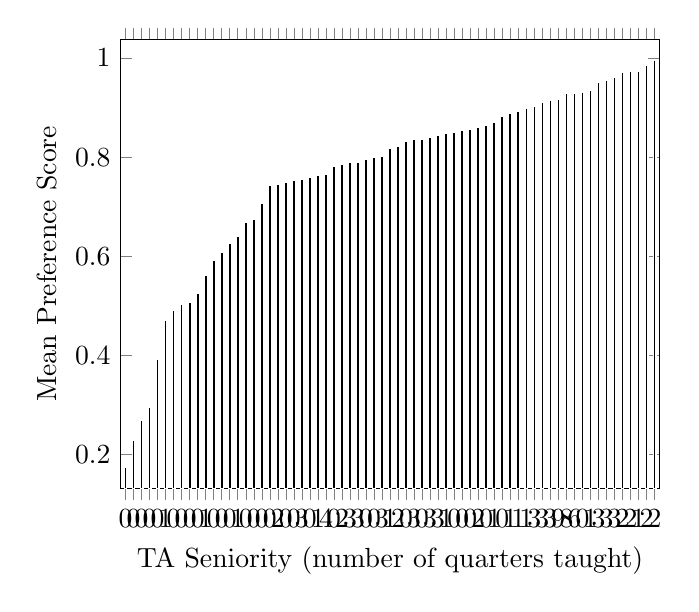
\begin{tikzpicture}
      \begin{axis}[
         ylabel=Mean Preference Score,
         xlabel=TA Seniority (number of quarters taught),
         bar width=1pt,
         enlarge x limits=0.01,
         enlarge y limits=0.05,
         ybar,
         xtick={0, 1, 2, 3, 4, 5, 6, 7, 8, 9, 10, 11, 12, 13, 14, 15, 16, 17, 18, 19, 20, 21, 22, 23, 24, 25, 26, 27, 28, 29, 30, 31, 32, 33, 34, 35, 36, 37, 38, 39, 40, 41, 42, 43, 44, 45, 46, 47, 48, 49, 50, 51, 52, 53, 54, 55, 56, 57, 58, 59, 60, 61, 62, 63, 64, 65, 66},
         xticklabels={0, 0, 0, 0, 0, 1, 0, 0, 0, 0, 1, 0, 0, 0, 1, 0, 0, 0, 0, 2, 0, 0, 3, 0, 1, 4, 0, 2, 3, 3, 0, 0, 3, 1, 2, 0, 3, 0, 3, 3, 1, 0, 0, 0, 2, 0, 1, 0, 1, 1, 1, 3, 3, 3, 9, 8, 6, 0, 1, 3, 3, 3, 2, 2, 1, 2, 2}
      ]
      \addplot+[draw=white, fill=black] coordinates
      {
(0, 0.17393224057428786)
(1, 0.22900763358778625)
(2, 0.26975259377494015)
(3, 0.29591836734693877)
(4, 0.39237451737451734)
(5, 0.47012987012987006)
(6, 0.49021029731689625)
(7, 0.5031446540880503)
(8, 0.5074626865671642)
(9, 0.5243764172335601)
(10, 0.5612903225806452)
(11, 0.5919377652050919)
(12, 0.6087420042643923)
(13, 0.6259878419452888)
(14, 0.6399515738498789)
(15, 0.6691729323308271)
(16, 0.6735449735449734)
(17, 0.7072743207712533)
(18, 0.7432432432432432)
(19, 0.7458427309912459)
(20, 0.7494505494505495)
(21, 0.753968253968254)
(22, 0.7545219638242894)
(23, 0.7594972594972594)
(24, 0.7633928571428572)
(25, 0.7653061224489796)
(26, 0.7810304449648712)
(27, 0.7857142857142857)
(28, 0.7889610389610389)
(29, 0.7896825396825395)
(30, 0.7959183673469388)
(31, 0.7990654205607477)
(32, 0.8009259259259259)
(33, 0.8174244314928725)
(34, 0.8221884498480243)
(35, 0.8317307692307692)
(36, 0.8347826086956522)
(37, 0.8349056603773585)
(38, 0.8389830508474576)
(39, 0.8443396226415094)
(40, 0.8485714285714285)
(41, 0.8489583333333333)
(42, 0.8530612244897959)
(43, 0.8560606060606061)
(44, 0.8597560975609756)
(45, 0.8640350877192983)
(46, 0.8701923076923077)
(47, 0.8828571428571428)
(48, 0.8879310344827587)
(49, 0.8926553672316384)
(50, 0.8979591836734694)
(51, 0.9013227513227513)
(52, 0.910828025477707)
(53, 0.9144869215291751)
(54, 0.9163265306122449)
(55, 0.9285714285714286)
(56, 0.9285714285714286)
(57, 0.9299363057324841)
(58, 0.9351851851851851)
(59, 0.9498556998556998)
(60, 0.9548872180451128)
(61, 0.961038961038961)
(62, 0.97)
(63, 0.9722222222222222)
(64, 0.9724770642201834)
(65, 0.9846153846153847)
(66, 0.9956896551724138)
      };
      \end{axis}
   \end{tikzpicture}
   \caption{\small{ Mean preference scores $x_{ij}a_{ij}$ for each TA in the LP generated schedule with $w = 1$ and $a_{min} = 0$. Because we give seniors priority, we observe that less experienced TAs (especially those with no or only 1 quarter of experience) get the worst assignments. While this schedule is optimal in terms of total weighted adherence, we recommend raising $a_{min}$ to a higher value so that assignments for TAs to the far left meet a more reasonable lower bound.}}
\end{figure*}

\begin{figure*}[ht]
   \centering
   \pgfplotsset{tick label style={font=\footnotesize},
      label style={font=\small},
      legend style={font=\small},
      width=14cm,
      height=7cm
   }
   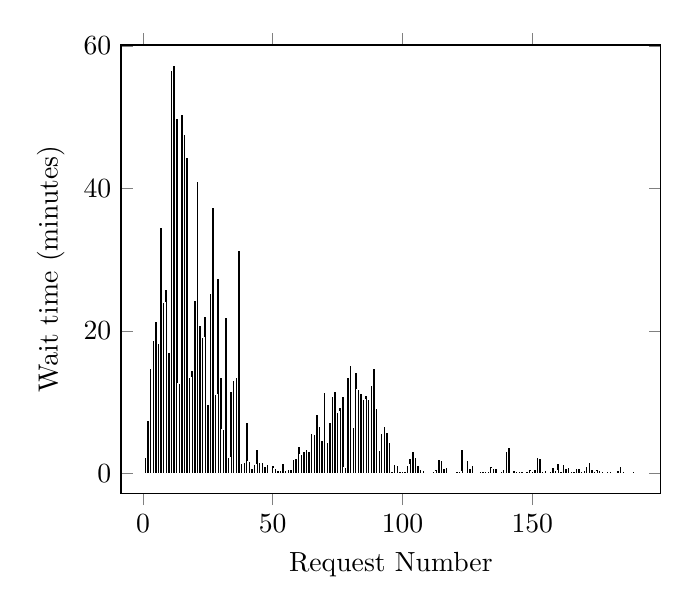
\begin{tikzpicture}
      \begin{axis}[
         ylabel=Wait time (minutes),
         xlabel=Request Number,
         bar width=1pt,
         enlarge x limits=0.05,
         enlarge y limits=0.05,
         ybar
      ]
      \addplot+[draw=white, fill=black] coordinates
      {(1, 2.3333333333333335) (2, 7.483333333333333) (3, 14.8) (4, 18.65) (5, 21.383333333333333) (6, 18.316666666666666) (7, 34.516666666666666) (8, 23.983333333333334) (9, 25.833333333333332) (10, 17.05) (11, 56.55) (12, 57.25) (13, 49.85) (14, 12.633333333333333) (15, 50.35) (16, 47.63333333333333) (17, 44.3) (18, 13.466666666666667) (19, 14.416666666666666) (20, 24.35) (21, 40.983333333333334) (22, 20.733333333333334) (23, 19.066666666666666) (24, 22.016666666666666) (25, 9.733333333333333) (26, 25.216666666666665) (27, 37.333333333333336) (28, 11.166666666666666) (29, 27.4) (30, 13.5) (31, 6.233333333333333) (32, 21.95) (33, 2.2333333333333334) (34, 11.466666666666667) (35, 13.083333333333334) (36, 13.483333333333333) (37, 31.35) (38, 1.4333333333333333) (39, 1.55) (40, 7.133333333333334) (41, 1.7333333333333334) (42, 0.7666666666666667) (43, 1.3) (44, 3.35) (45, 1.6166666666666667) (46, 1.6) (47, 1.0166666666666666) (48, 1.3333333333333333) (49, 0.13333333333333333) (50, 1.1) (51, 0.7166666666666667) (52, 0.5166666666666667) (53, 0.45) (54, 1.3833333333333333) (55, 0.4666666666666667) (56, 0.6) (57, 0.5333333333333333) (58, 1.9333333333333333) (59, 2.1) (60, 3.8833333333333333) (61, 2.75) (62, 3.1) (63, 3.4166666666666665) (64, 3.1666666666666665) (65, 5.666666666666667) (66, 5.45) (67, 8.25) (68, 6.633333333333334) (69, 4.7) (70, 11.333333333333334) (71, 4.4) (72, 7.133333333333334) (73, 10.9) (74, 11.6) (75, 8.65) (76, 9.25) (77, 10.816666666666666) (78, 0.8666666666666667) (79, 13.516666666666667) (80, 15.15) (81, 6.45) (82, 14.133333333333333) (83, 11.866666666666667) (84, 11.216666666666667) (85, 10.466666666666667) (86, 11.016666666666667) (87, 10.383333333333333) (88, 12.433333333333334) (89, 14.816666666666666) (90, 9.2) (91, 3.2333333333333334) (92, 5.583333333333333) (93, 6.633333333333334) (94, 5.833333333333333) (95, 4.45) (96, 0.3333333333333333) (97, 1.3) (98, 1.1666666666666667) (99, 0.25) (100, 0.36666666666666664) (101, 0.25) (102, 1.2166666666666666) (103, 2.15) (104, 3.183333333333333) (105, 2.283333333333333) (106, 1.1833333333333333) (107, 0.65) (108, 0.43333333333333335) (109, 0.23333333333333334) (110, 0.21666666666666667) (111, 0.18333333333333332) (112, 0.3) (113, 0.5333333333333333) (114, 1.95) (115, 1.8833333333333333) (116, 0.7) (117, 0.8166666666666667) (118, 0.15) (119, 0.21666666666666667) (120, 0.1) (121, 0.31666666666666665) (122, 0.26666666666666666) (123, 3.45) (124, 0.2) (125, 1.8333333333333333) (126, 0.7) (127, 1.1666666666666667) (128, 0.18333333333333332) (129, 0.2) (130, 0.25) (131, 0.38333333333333336) (132, 0.2833333333333333) (133, 0.35) (134, 1.0333333333333334) (135, 0.7333333333333333) (136, 0.6666666666666666) (137, 0.21666666666666667) (138, 0.31666666666666665) (139, 0.5333333333333333) (140, 3.1333333333333333) (141, 3.75) (142, 0.21666666666666667) (143, 0.5166666666666667) (144, 0.31666666666666665) (145, 0.25) (146, 0.31666666666666665) (147, 0.18333333333333332) (148, 0.3) (149, 0.6333333333333333) (150, 0.26666666666666666) (151, 0.55) (152, 2.316666666666667) (153, 2.1666666666666665) (154, 0.26666666666666666) (155, 0.43333333333333335) (156, 0.23333333333333334) (157, 0.3333333333333333) (158, 0.8666666666666667) (159, 0.4) (160, 1.45) (161, 0.3333333333333333) (162, 1.25) (163, 0.7166666666666667) (164, 0.8833333333333333) (165, 0.26666666666666666) (166, 0.38333333333333336) (167, 0.6833333333333333) (168, 0.75) (169, 0.35) (170, 0.4) (171, 0.9666666666666667) (172, 1.6333333333333333) (173, 0.6333333333333333) (174, 0.3333333333333333) (175, 0.55) (176, 0.4666666666666667) (177, 0.31666666666666665) (178, 0.2) (179, 0.25) (180, 0.25) (181, 0.13333333333333333) (182, 0.21666666666666667) (183, 0.4) (184, 1.0666666666666667) (185, 0.25) (186, 0.16666666666666666) (187, 0.21666666666666667) (188, 0.13333333333333333) (189, 0.25) (190, 0.21666666666666667)
};
      \end{axis}
   \end{tikzpicture}
   \caption{\small{Real queue response time across the first Thursday of the Autumn 2014 term (Oct. 2nd), one of the first busy days of the term. Requests are sorted horizontally by request time, and queue wait time is plotted in real time minutes.}}
\end{figure*}

\begin{figure*}[ht]
   \centering
   \pgfplotsset{tick label style={font=\footnotesize},
      label style={font=\small},
      legend style={font=\small},
      width=14cm,
      height=7cm
   }
   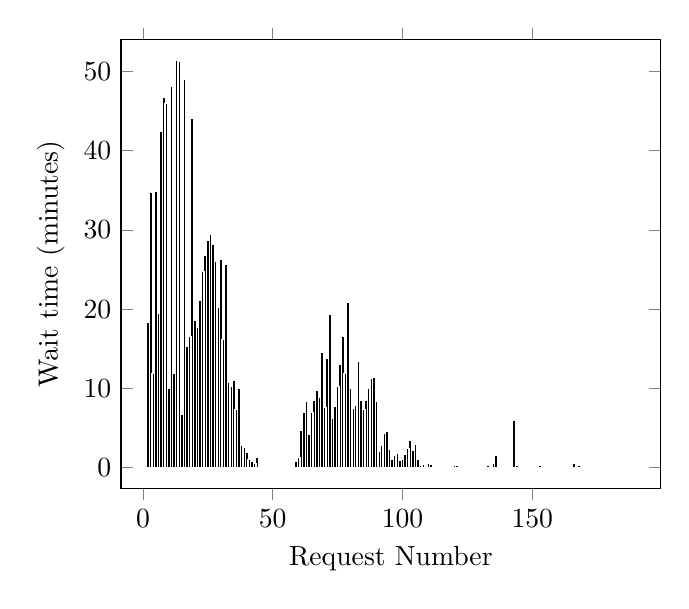
\begin{tikzpicture}
      \begin{axis}[
         ylabel=Wait time (minutes),
         xlabel=Request Number,
         bar width=1pt,
         enlarge x limits=0.05,
         enlarge y limits=0.05,
         ybar
      ]
      \addplot+[draw=white, fill=black] coordinates
      {(1, 0.010977203883495141) (2, 18.308932077669905) (3, 34.76826384466022) (4, 11.888447242718446) (5, 34.8259767378641) (6, 19.41781176699029) (7, 42.450211048543686) (8, 46.73081813592232) (9, 45.90933658252427) (10, 10.044956970873786) (11, 48.14972161165046) (12, 11.897623223300975) (13, 51.43342753398057) (14, 51.207098330097054) (15, 6.695578485436894) (16, 49.01235431067964) (17, 15.265852427184468) (18, 16.54027654368932) (19, 44.116518932038844) (20, 18.542209106796115) (21, 17.644338000000005) (22, 21.08994221359223) (23, 24.70971669902913) (24, 26.82062108737864) (25, 28.655825941747572) (26, 29.40743516504855) (27, 28.19843056310679) (28, 25.987985650485435) (29, 20.178571281553396) (30, 26.306993359223302) (31, 16.13289355339804) (32, 25.635190368932026) (33, 10.822644349514567) (34, 10.220503281553398) (35, 11.03271972815534) (36, 7.299512038834951) (37, 9.954634194174755) (38, 2.8284093786407776) (39, 2.5616313786407767) (40, 1.8735364660194187) (41, 1.0511503689320392) (42, 0.8054030097087399) (43, 0.51021227184466) (44, 1.3021584466019411) (45, 0.011277262135925566) (46, 0.08997815533980762) (47, 0.012799223300972006) (48, 0.007703126213595311) (49, 0.01037132038835097) (50, 0.009895980582526054) (51, 0.010725029126215533) (52, 0.009642058252430743) (53, 0.009688893203884953) (54, 0.009023941747571682) (55, 0.04286079611650712) (56, 0.010342834951455177) (57, 0.011348912621358094) (58, 0.013738543689322823) (59, 0.792714058252426) (60, 1.2831023883495152) (61, 4.743866097087379) (62, 6.9657686213592225) (63, 8.369605223300972) (64, 4.146125592233009) (65, 6.958186601941748) (66, 8.54442401941748) (67, 9.791618504854368) (68, 8.853189378640776) (69, 14.537343145631063) (70, 7.573002116504856) (71, 13.795429631067964) (72, 19.29489833009709) (73, 6.168550893203883) (74, 7.788167475728157) (75, 10.216771165048543) (76, 13.030464233009706) (77, 16.52000959223301) (78, 11.863840893203877) (79, 20.821164640776697) (80, 10.031464135922329) (81, 7.496020310679612) (82, 7.835424116504854) (83, 13.369403184466016) (84, 8.435309766990292) (85, 7.376770485436889) (86, 8.450645766990293) (87, 9.949425902912623) (88, 11.252177300970866) (89, 11.335158873786407) (90, 8.38442813592233) (91, 2.0548223300970876) (92, 2.818756834951456) (93, 4.324656407766992) (94, 4.592855359223298) (95, 2.268767533980582) (96, 1.021327339805825) (97, 1.5443984271844673) (98, 1.8635569514563113) (99, 0.9132338446601942) (100, 1.0313365631067943) (101, 1.6520130873786405) (102, 2.4374074368932046) (103, 3.469509436893204) (104, 2.174446135922329) (105, 2.8915217475728165) (106, 1.0789088155339803) (107, 0.3086196116504862) (108, 0.38789598058252733) (109, 0.1684347378640791) (110, 0.5899190679611643) (111, 0.4066682330097099) (112, 0.008551048543691264) (113, 0.007175533980583982) (114, 0.007454796116507443) (115, 0.007710116504854691) (116, 0.009883922330099515) (117, 0.06079194174757555) (118, 0.007838038834952269) (119, 0.12730666019417816) (120, 0.2662130097087368) (121, 0.24162238834951746) (122, 0.008333300970877346) (123, 0.008293106796117476) (124, 0.007573805825244336) (125, 0.007832446601939158) (126, 0.007868271844662137) (127, 0.008048621359225565) (128, 0.007681805825243041) (129, 0.007650524271843204) (130, 0.007624834951458899) (131, 0.007854466019420069) (132, 0.007817941747571198) (133, 0.31861625242718483) (134, 0.05776968932039046) (135, 0.5727481165048556) (136, 1.5425792038834942) (137, 0.007447281553398383) (138, 0.007699805825241906) (139, 0.009626504854370391) (140, 0.006952368932042556) (141, 0.007861456310673625) (142, 0.021051611650482204) (143, 5.992825456310679) (144, 0.34436900970873957) (145, 0.00735815533980971) (146, 0.00802922330096764) (147, 0.0073518640776678015) (148, 0.008241902912624431) (149, 0.0070584466019472485) (150, 0.007420543689320552) (151, 0.00686254368931958) (152, 0.007579048543681878) (153, 0.23594644660194275) (154, 0.007091825242720547) (155, 0.007656466019415694) (156, 0.007133766990295796) (157, 0.007839786407766993) (158, 0.007383320388348869) (159, 0.007018427184477187) (160, 0.007234252427183657) (161, 0.007545669902909066) (162, 0.007147747572813274) (163, 0.006568601941744662) (164, 0.01761763106796375) (165, 0.015898543689320713) (166, 0.4814839223300971) (167, 0.10302483495145222) (168, 0.23662537864077796) (169, 0.007164349514560677) (170, 0.007764815533990452) (171, 0.007599844660194179) (172, 0.007002000000002591) (173, 0.007703650485434304) (174, 0.006694252427180579) (175, 0.007418970873782043) (176, 0.007440116504849997) (177, 0.007585339805823784) (178, 0.007467728155342557) (179, 0.006896970873789645) (180, 0.007449029126217149) (181, 0.00752172815534207) (182, 0.007212407766995794) (183, 0.007428407766991103) (184, 0.007013533980583821) (185, 0.007010737864079449) (186, 0.00702489320388366) (187, 0.006787398058256153) (188, 0.006671883495143202) (189, 0.0068455922330144005) (190, 0.008386077669905833)};
      \end{axis}
   \end{tikzpicture}
   \caption{\small{Simulation results for the same day as in Figure 3. Response times are averages from 100 simulation runs, each of which was run at 1,080x real time. Differences between observed and simulation wait times are likely the result of oversimplifications in our simulated dequeue and service policies.}}
\end{figure*}

\end{multicols}
\end{document}
